\documentclass[12pt]{article}
\usepackage{amsmath,amssymb,amsfonts,amsthm}
\usepackage{geometry}
\usepackage{setspace}      % For double spacing
% \usepackage{mathptmx}      % Times New Roman font
\usepackage{physics}
\usepackage[hidelinks]{hyperref}
\usepackage{color}
\usepackage{xcolor}
\usepackage{subcaption}
\usepackage{tikz}
\usepackage{tikz-3dplot}
\usetikzlibrary{backgrounds, intersections}
\usetikzlibrary{calc}
\usetikzlibrary{math}
\usetikzlibrary{shapes.geometric}
\usepackage{pgfplots}
\usepackage{enumitem}
\usepackage{xcolor}

\pgfplotsset{compat=1.18}

\geometry{margin=1in}

% Set double spacing
\setstretch{1.5}

\newcommand{\todo}[1]{\textcolor{red}{#1}}
\newcommand{\note}[1]{\textcolor{blue}{#1}}

\newcommand{\R}{\mathbb{R}}
\newcommand{\C}{\mathbb{C}}
\newcommand{\Z}{\mathbb{Z}}
\newcommand{\N}{\mathbb{N}}
\newcommand{\Q}{\mathbb{Q}}
\newcommand{\F}{\mathbb{F}}


% Define global parameters and common drawing commands:
\pgfmathsetmacro{\dominio}{2.0}    % Height of the cylinder
\pgfmathsetmacro{\radio}{1}        % Radius of the cylinder
\pgfmathsetmacro{\step}{\dominio/70.0}

% Macro to draw the common 3D coordinate axes.
\newcommand{\drawAxes}{
  \draw[thick,->] (0,0,0) -- (0,2,0) node[above] {$z$};
  \draw[thick,->] (0,0,0) -- (1.8,0,0) node[right] {$x$};
  \draw[thick,->] (0,0,0) -- (-1.8,0,0) node[left] {$-x$};
  \draw[thick,->] (0,0,0) -- (0,0,2) node[above] {$-y$};
  \draw[thick,->] (0,0,0) -- (0,0,-2) node[below] {$y$};
}

% Macro to draw the cylinder using circular slices along the z-axis.
\newcommand{\drawCylinder}{
  \foreach \z in {0,\step,...,\dominio} {
    \draw[cyan,very thick,opacity=0.35]
	  plot[domain=0:360,smooth,variable=\t]
	  ({\radio*cos(\t)}, {\z}, {\radio*sin(\t)});
  }
}

\newcommand{\drawsphere}{
	\shade[ball color = cyan!40, opacity = 0.65] (0,0) circle (1.5cm);
	\draw (0,0) circle (1.5cm);
}


\tdplotsetmaincoords{60}{130}     % your camera
\tdplotsetrotatedcoords{35}{-45}{0}  % so that the plane is z'=0


\newtheorem{definition}{Definition}[section]
\newtheorem{theorem}[definition]{Theorem}
\newtheorem{proposition}[definition]{Proposition}
\newtheorem{corollary}[definition]{Corollary}

\geometry{margin=1in}
\title{Geodesics, Symmetries, and Isometries:\\A Comprehensive Study and Applications}
\author{Ulizes Raudales}
\date{\today}

\begin{document}
\maketitle

\newpage
\tableofcontents
\newpage

\begin{abstract}
	This thesis develops a unified framework for geodesic analysis on smooth surfaces in \(\R^3\) and in the Schwarzschild spacetime, showing how continuous symmetries give rise to conserved quantities via Killing vector fields and Noether’s theorem.  
	We derive the general geodesic equations, specialize to surfaces of revolution to obtain Clairaut’s relation with concrete examples, and present practical methods for identifying and exploiting isometries.  
	Applying these techniques to the Schwarzschild metric, we obtain the effective potential for null and time-like geodesics and characterize circular orbits and the photon sphere.
\end{abstract}

\section{Introduction}
Geodesics—curves that locally minimize distance or more accurate, the "straightest" line in a curved surface, play a fundamental role in both theoretical and applied contexts.  
On the Earth’s surface, they describe great‐circle routes used in air and sea navigation, enabling efficient path planning across long distances.  
In computer graphics and mesh processing, geodesic computations underpin texture mapping, shape interpolation, and shortest‐path queries on complex surfaces.  
In robotics, geodesic algorithms guide motion planning over uneven terrains and within configuration spaces to avoid obstacles while minimizing energy or time.

Beyond these engineering applications, geodesics are central to our understanding of gravity in Einstein’s theory of general relativity.  
Free‐falling particles and light rays follow spacetime geodesics, so that phenomena such as gravitational lensing, perihelion precession, and black‐hole photon spheres can be analyzed through purely geometric methods.  
This deep connection between curvature and motion has inspired techniques ranging from GPS corrections in satellite orbits to simulations of cosmological structure formation.

Motivated by this wide-ranging importance, the present thesis develops a systematic framework for deriving and solving geodesic equations on smooth surfaces in \(\R^3\) and on the Schwarzschild spacetime.  
By identifying continuous symmetries and their associated Killing vector fields, we obtain conserved quantities that greatly simplify both theoretical analysis and numerical implementation.  The methods presented here provide a unified toolkit for applications in geodesy, graphics, robotics, and gravitational physics.

\section{Background and Preliminaries}

Differential geometry is a branch of mathematics that uses the techniques of calculus and algebra to study problems in geometry. 
It is a field that has applications in many areas, including physics, engineering, and computer science.
In this section, we will introduce some of the basic concepts and tools that will be used throughout this thesis. 

\subsection{Surfaces in \texorpdfstring{$\mathbb{R}^3$}{R3}}\label{sec:surface-def}

In differential geometry, an $n$-dimensional \emph{manifold} is a topological space that is locally resembles $\mathbb{R}^n$, n-dimensional Euclidean space. 
We will focus on \emph{surfaces}, which are 2-dimensional manifolds embedded, i.e., smoothly and continuously mapped, in $\mathbb{R}^3$.
The embedding in $\mathbb{R}^3$ endows the surface with additional geometric structure (coming from the ambient Euclidean geometry) that allows us to measure distances, angles, and curvature.

\begin{definition}[Surface]\label{def:surface}
	A regular surface $\mathcal{S}\subset\R^3$ is the image of a one-to-one smooth map that maps an open set $U\subset\R^{2}$ into $\R^3$:
	\begin{equation}\label{eq:surface-param}		
		\mathbf{r}: U\subset\R^{2}\to\R^3 \qquad \mathbf{r}(u,v) = \begin{bmatrix}
			x(u,v)\\[1ex]
			y(u,v)\\[1ex]
			z(u,v)
		\end{bmatrix}
	\end{equation}
	with $\mathbf{r}$ being regular(i.e., $\pdv{\mathbf{r}}{u} \times \pdv{\mathbf{r}}{v} \neq 0$ for all $(u,v)\in U$).
\end{definition}

For clarity, denote the surface by $\mathcal{S}=\mathbf{r}(U)$. At any point $\mathbf{r}(u_0,v_0)$, the tangent vectors are given by
\[
\mathbf{r}_u = \pdv{\mathbf{r}}{u}, \quad \mathbf{r}_v = \pdv{\mathbf{r}}{v},
\]
which span the tangent plane at some point $p = \mathbf{r}(u_0,v_0)$, that is 
\[
T_{p}(\mathcal{S}) = \text{span}\{\mathbf{r}_u,\mathbf{r}_v\}.
\]
where $T_{p}(\mathcal{S})$ is the tangent space at point $p$.
So by definition, for any tanget vector $\mathbf{v}\in T_{p}(\mathcal{S})$, we can write
\[
\mathbf{v} = a\mathbf{r}_u + b\mathbf{r}_v,
\]
where $a,b\in\R$ are real numbers.

We have that the unit normal vector $\mathbf{U}$ to the surface at point $p$ is given by
\[
\mathbf{U} = \frac{\mathbf{r}_u\times\mathbf{r}_v}{\|\mathbf{r}_u\times\mathbf{r}_v\|}.
\]
which is a unit vector orthogonal to the tangent plane at point $p$.

\subsection{The Metric on a Surface}
A property of surfaces is that they are metric spaces, meaning that they come with a metric that allows us to measure distances and angles.
The \emph{metric}, which is a smoothly varying inner product on the tangent plane at each point allows us to measure lengths of curves, angles between tangent vectors, and surface areas. 
For an embedded surface with local coordinates $(u,v)$, the metric (also called the \emph{first fundamental form}) can be obtained by restricting the Euclidean dot product to the tangent plane:
\[
g_{\,\mu\nu} = \mathbf{r}_\mu\,\cdot\,\mathbf{r}_\nu, \qquad \mu,\nu \in \{u,v\}.
\]
In matrix form, the metric tensor can be written as 
\[
g_{\mu\nu} = 
\begin{bmatrix}
E & F\\[1ex]
F & G
\end{bmatrix},
\] 
where 
\begin{equation}\label{eq:metric-coefficients}
	E = \mathbf{r}_u\cdot \mathbf{r}_u, \qquad F = \mathbf{r}_u\cdot \mathbf{r}_v, \qquad G = \mathbf{r}_v\cdot \mathbf{r}_v.
\end{equation}

Thus, for an infinitesimal displacement $dq = (du,\;dv)^\top$ in the parameter domain, the squared distance traveled on the surface is 
\begin{equation}\label{eq:line-element}
ds^{2} \;=\; \begin{bmatrix}
	E & F\\[1ex]
	F & G
\end{bmatrix} \begin{bmatrix}
	du\\[1ex]
	dv
\end{bmatrix} \cdot \begin{bmatrix}
	du\\[1ex]
	dv
\end{bmatrix} \;=\; E\,du^{2} + 2F\,du\,dv + G\,dv^{2}.
\end{equation}
This is the \emph{line element} of the surface, which describes how distances are measured on the surface.

We find the length of the line element by the following:
\[
	L = \int_{a}^{b} \sqrt{ds^{2}} dt
\]

\subsection{Curves on a Surface}
With the metric in hand, we can consider curves drawn on the surface and measure their lengths. 

\begin{definition}[Curve on a Surface]\label{def:curve}
A (parametrized) curve $\gamma$ on a surface $\mathcal{S}$ is a smooth map $\gamma: I \to \mathcal{S}$ from an interval $I\subset \mathbb{R}$ into the surface. 
Writing 
\begin{equation}\label{eq:curve-param}
	\gamma(t) = \mathbf{r}(u(t), v(t))
\end{equation}
in terms of a local parametrization of $\mathcal{S}$, the coordinates $(u(t), v(t))$ describe the path of the curve in the parameter domain. 
\end{definition}
The velocity (tangent) vector of $\gamma$ at parameter $t$ is 
\begin{equation}\label{eq:curve-vel}
	\dot\gamma(t) = \frac{d}{dt}\mathbf{r}(u(t), v(t)) = \dot{u}(t)\,\mathbf{r}_u + \dot{v}(t)\,\mathbf{r}_v,
\end{equation}
which indeed lies in the tangent plane $T_{\gamma(t)}(\mathcal{S})$. 


\begin{definition}[Unit Speed Curve]\label{def:unit-speed}
A curve $\gamma(t)$ on $\mathcal{S}$ is \emph{unit speed} (or parametrized by arc length) if the following condition holds for all $t$:
\[
\|\dot{\gamma}(t)\|^{2} = 1
\] 
\end{definition}

Under this condition, the parameter $t$ itself represents the arc length along the curve. 


\subsection{Arc Length Reparametrization}
Any regular curve $\gamma(t)$ can be reparametrized to have unit speed (except at points where $\dot\gamma=0$). 
This is done by defining a new parameter $s$ as the arc length from some fixed point $t_0$ to $t$:
\[
s(t) = \int_{t_0}^{t} \|\dot\gamma(t)\|\,dt 
\]
By the Fundamental Theorem of Calculus, we have that $\dot{s}(t) = \|\dot\gamma(t)\| > 0$.
By the Mean Value Theorem, $s(t)$ is a strictly increasing function of $t$ and thus has an inverse function $t(s)$.
Now define a new curve \(\beta(s)\) by reparameterizing \(\gamma(t)\) with respect to the arc length \(s\):
\[
\beta(s)=\gamma(t(s)).
\]
We can show that \(\beta(s)\) is a unit speed curve.
By the chain rule,
\[
\dv{s}\beta(s) = \frac{d}{ds}\gamma(t(s)) = \gamma'(t(s))\,\frac{dt}{ds}.
\]
where 
\[
\frac{dt}{ds} = \frac{1}{\|\gamma'(t(s))\|}.
\]
Substitute the expression for \(\frac{dt}{ds}\) into the derivative of \(\beta(s)\),
\[
\dv{s}\beta(s) = \gamma'(t(s))\cdot \frac{1}{\|\gamma'(t(s))\|}.
\]
Taking the norm of both sides,
\[
\left\|\dv{s}\beta(s)\right\| = \left\|\gamma'(t(s)) \cdot \frac{1}{\|\gamma'(t(s))\|}\right\| = \frac{\|\gamma'(t(s))\|}{\|\gamma'(t(s))\|} = 1.
\]
Therefore, all curves can be reparameterized to have unit speed.

Under arc length reparametrization, we call $s$ the \emph{arc length parameter} or \emph{proper time} in the context of general relativity.
This parameter is usually refered as the \emph{affine parameter} in the context of geodesics, as it is a parameter that preserves the affine structure of the curve.
Affine parameters are exactly those parameters for which the geodesic equation has no extra “forcing” term.

\subsection{Curvature of curves}
The curvature of a curve is a measure of how much the curve deviates from being a straight line.
In Euclidean space, the curvature of a curve is defined as the rate of change of the tangent vector with respect to the arc length parameter.

\begin{definition}[Curvature]\label{def:curvature}
	The curvature of a curve $\gamma(t)$ is defined as
	\[
	\kappa_{\gamma} = \frac{\|\dot{\gamma}\times\ddot{\gamma}\|}{\|\dot{\gamma}\|^{3}}.
	\]
	For a unit speed curve, this simplifies to
	\[
	\kappa_{\beta}(s) = \|\ddot{\beta}(s)\|.
	\]
\end{definition}
The curvature is a scalar quantity that describes how much the curve bends at a given point.

Another important quantity related to curvature is the normal curvature, which is the projecction of the curvature vector onto the normal vector of the surface at that point.
\[
	\kappa_{\mathbf{N}} = \mathbf{N} \cdot \kappa_{\gamma}
\]
The normal curvature is a measure of how much the curve bends in the direction of the normal vector at that point.


\section{Geodesics}
% When working on surfaces, we want to find the "straightest" paths between two points on the surface, which are usually the shortest paths.
% In Euclidean space, the straightest path between two points is a straight line.
% However, on a curved surface, the shortest path may not be a straight line in the Euclidean sense.

Another important quantity related to curvature is the \emph{geodesic curvature}, which is how much the curve deviates from being a geodesic on the surface.
Which is defined as 
\begin{equation}\label{eq:geodesic-curvature}
	\kappa_{g} = \kappa_{\gamma} - \kappa_{\mathbf{N}}.
\end{equation}

A geodesic can also be thought as the shortest path between two points on a surface.
However, this is not always the case, as shown in \cite{jia2024geodesics} and will be discussed in more detail once we explore geodesics on different surfaces.

\begin{definition}[Geodesic]\label{def:geodesic}
	A curve $\gamma(t)$ on a surface $\mathcal{S}$ or any manifold $\mathcal{M}$ is called a \emph{geodesic} if it is the "straightest" path between two points on the surface.
	More formally, a curve is a geodesic if it has zero geodesic curvature:
	\[
	\kappa_{g} = 0.
	\]
\end{definition}

\subsection{Deriving the Geodesic Equation}

To find the geodesics of a surface, we let $\gamma(t)$ be a geodesic on a surface $\mathcal{S}$; the curve parameterized in terms of Eq.(\ref{eq:curve-param}) and find its velocity vector Eq.(\ref{eq:curve-vel}).
We can also find the acceleration vector of the curve by differentiating the velocity vector with respect to $t$:
\begin{equation}\label{eq:curve-acc}
	\ddot\gamma(t) = \dot{u}(t)^{2}\mathbf{r}_{uu} + \dot{v}(t)^{2}\mathbf{r}_{vv} + 2\dot{u}(t)\dot{v}(t)\mathbf{r}_{uv} + \ddot{u}\mathbf{r}_{u} + \ddot{v}\mathbf{r}_{v}.
\end{equation}

We can break $\ddot{\gamma}(t)$ into two components: the tangential component to the surface and the normal component to the surface.
\begin{equation}\label{eq:curve-acc-decomp}
	\ddot{\gamma}(t) = \ddot{\gamma}_{\text{norm}}(t) + \ddot{\gamma}_{\text{tan}}(t),
\end{equation}

The normal component, $\ddot{\gamma}_{\text{norm}}(t)$, is the curvature imposed by the surface on the curve, while the tangential component, $\ddot{\gamma}_{\text{tan}}(t)$, is any extra curvature imposed by the curve itself.
We thus have
\[
	\kappa_{g} = \ddot{\gamma}_{\text{tan}}(t) \cdot \mathbf{U} = 0,
\]
The derivation for rhe tangential component of the acceleration vector is outside the scope of this thesis, but its derivation can be found in \cite{celano2022why}\cite{oprea2007differential}, so we have 
\[
	\ddot{\gamma}_{\text{tan}}(t) = \ddot{\gamma} \cdot \mathbf{r}_{u} + \ddot{\gamma} \cdot \mathbf{r}_{v} = 0.
\]
Since we want the geodesic curvature to be zero, and since both components are linearly independent, the dot products cannot be additive inverses of each other, so we can set them to zero:
\[
	\ddot{\gamma}(t) \cdot \mathbf{r}_{u} = 0, \qquad \ddot{\gamma}(t) \cdot \mathbf{r}_{v} = 0.
\]	
Substituting the expression for $\ddot{\gamma}(t)$ from Eq.(\ref{eq:curve-acc}) into these two equations gives us two second-order ordinary differential equations for $u(t)$ and $v(t)$:
\begin{align*}
	\ddot{\gamma} \cdot \mathbf{r}_{u} = \dot{u}(t)^{2}\mathbf{r}_{uu} \cdot \mathbf{r}_{u} + \dot{v}(t)^{2}\mathbf{r}_{vv} \cdot \mathbf{r}_{u} + 2\dot{u}(t)\dot{v}(t)\mathbf{r}_{uv} \cdot \mathbf{r}_{u} + \ddot{u}\mathbf{r}_{u} \cdot \mathbf{r}_{u} + \ddot{v}\mathbf{r}_{v} \cdot \mathbf{r}_{u} = 0 \\
	\ddot{\gamma} \cdot \mathbf{r}_{v} = \dot{u}(t)^{2}\mathbf{r}_{uu} \cdot \mathbf{r}_{v} + \dot{v}(t)^{2}\mathbf{r}_{vv} \cdot \mathbf{r}_{v} + 2\dot{u}(t)\dot{v}(t)\mathbf{r}_{uv} \cdot \mathbf{r}_{v} + \ddot{u}\mathbf{r}_{u} \cdot \mathbf{r}_{v} + \ddot{v}\mathbf{r}_{v} \cdot \mathbf{r}_{v} = 0. 
\end{align*}
Because $\mathbf{r}_{u}$ and $\mathbf{r}_{v}$ are orthogonal and thus $\mathbf{r}_{u}\cdot\mathbf{r}_{v} = 0$, and isolating the second derivatives gives us the following two equations:
\begin{align}
	\ddot{u} + \dot{u}(t)^{2}\frac{\mathbf{r}_{uu} \cdot \mathbf{r}_{u}}{\mathbf{r}_{u} \cdot \mathbf{r}_{u}} + \dot{v}(t)^{2}\frac{\mathbf{r}_{vv} \cdot \mathbf{r}_{u}}{\mathbf{r}_{u} \cdot \mathbf{r}_{u}} + 2\dot{u}(t)\dot{v}(t)\frac{\mathbf{r}_{uv} \cdot \mathbf{r}_{u}}{\mathbf{r}_{u} \cdot \mathbf{r}_{u}} = 0 \label{eq:geodesic-acc-decomp-1}\\
	\ddot{v} + \dot{u}(t)^{2}\frac{\mathbf{r}_{uu} \cdot \mathbf{r}_{v}}{\mathbf{r}_{v} \cdot \mathbf{r}_{v}} + \dot{v}(t)^{2}\frac{\mathbf{r}_{vv} \cdot \mathbf{r}_{v}}{\mathbf{r}_{v} \cdot \mathbf{r}_{v}} + 2\dot{u}(t)\dot{v}(t)\frac{\mathbf{r}_{uv} \cdot \mathbf{r}_{v}}{\mathbf{r}_{v} \cdot \mathbf{r}_{v}} = 0. \label{eq:geodesic-acc-decomp-2}
\end{align}
Recall that by Eq.(\ref{eq:metric-coefficients}), we have
\[
	E = \mathbf{r}_{u} \cdot \mathbf{r}_{u}  \qquad F = \mathbf{r}_{u} \cdot \mathbf{r}_{v} \qquad G = \mathbf{r}_{v} \cdot \mathbf{r}_{v}\\
\]
Taking the derivatives of each coefficient with respect to $u$ and $v$ gives us the following relationships:
\begin{alignat*}{4}
E_{u} \; &=\; 2\,\mathbf{r}_{uu}\cdot \mathbf{r}_{u} \quad &\quad E_{v} \; &=\; 2\,\mathbf{r}_{uv}\cdot \mathbf{r}_{u}\\[5pt]
F_{u} \; &=\; \mathbf{r}_{uu}\cdot \mathbf{r}_{v} + \mathbf{r}_{u}\cdot \mathbf{r}_{uv} \quad &\quad F_{v} \; &=\; \mathbf{r}_{uv}\cdot \mathbf{r}_{v} + \mathbf{r}_{u}\cdot \mathbf{r}_{vv}\\[5pt]
G_{u} \; &=\; 2\,\mathbf{r}_{vu}\cdot \mathbf{r}_{v} \quad &\quad G_{v} \; &=\; 2\,\mathbf{r}_{vv}\cdot \mathbf{r}_{v}
\end{alignat*}
Substituting these relationships into the equations (\ref{eq:geodesic-acc-decomp-1}) and (\ref{eq:geodesic-acc-decomp-2}) gives us the following two equations:
\begin{equation}\label{eq:geodesic-uv}
	\ddot{u} + \frac{E_{u}}{2E}\dot{u}^{2} + 2\frac{E_{v}}{2E}\dot{u}\dot{v} - \frac{G_{u}}{2E}\dot{v}^{2} = 0
\end{equation}
\begin{equation}\label{eq:geodesic-vu}
	\ddot{v} - \frac{E_{v}}{2G}\dot{u}^{2} + 2\frac{G_{u}}{2G}\dot{u}\dot{v} + \frac{G_{v}}{2G}\dot{v}^{2} = 0
\end{equation}

These two equations are the geodesic equations for the coordinates \(u\) and \(v\) on the surface.
These equations correspond to the case where $F = 0$, as the equations are independent of the cross term $F$.
For our look at surfaces of revolution, we have that $F = 0$, as the surface is symmetric about the axis of rotation.
Hence, these are the geodesic equations we will be using for the rest of this thesis.

In the case where $F \neq 0$, we can write the geodesic equations in a more general form:
\begin{equation}\label{eq:geodesic-compact}
	\dv[2]{q^\sigma}{t} + \sum_{\mu,\nu=1}^{n} \Gamma_{\mu\nu}^\sigma \dv{q^\mu}{t} \dv{q^\nu}{t} = 0,
\end{equation}
where $n$ is the number of coordinates on the surface, and $q^\sigma$ are the coordinates on the surface.
$\Gamma_{\mu\nu}^\sigma$ are the \emph{Christoffel symbols} of the second kind, which describe how the metric changes as we move along the surface.
In our case of equations (\ref{eq:geodesic-uv}) and (\ref{eq:geodesic-vu}), we have
\[
\begin{aligned}
    \Gamma_{11}^{1} &= \frac{E_{u}}{2E} &\quad \Gamma_{12}^{1} &= \Gamma_{21}^{1} = \frac{E_{v}}{2E} &\quad \Gamma_{22}^{1} &= -\frac{G_{u}}{2E} \\[4mm]
    \Gamma_{11}^{2} &= -\frac{E_{v}}{2G} &\quad \Gamma_{12}^{2} &= \Gamma_{21}^{2} = \frac{G_{u}}{2G} &\quad \Gamma_{22}^{2} &= -\frac{G_{v}}{2G}.
\end{aligned}
\]

\section{Geodesics on Surfaces}

\subsection{Geodesics on Surfaces of Revolution}

Surfaces of revolution are a class of surfaces obtained by rotating a planar curve about an axis in the plane. 
They are highly symmetric surfaces, exhibiting rotational symmetry.

\begin{figure}[ht]
	\centering
	\begin{minipage}{0.48\textwidth}
	    \centering
		\begin{tikzpicture}[scale=1.2]
			\tikzmath{function f(\t) {return 1.5 + 0.35*sin(\t r);};}
			% Axes in the xz-plane
			\draw[->] (-2,0) -- (2,0) node[right] {$x$};
			\draw[->] (0,-2) -- (0,2) node[above] {$z$};
			\draw[dashed] (0,1) -- (1.8,1) node[midway, above] {$x(u)$};
			\draw[dashed] (1.8,0) -- (1.8,1) node[midway, right] {$z(u)$};

			% Plot of the profile curve: x = f(t), z = t
			\draw[domain=-2:2, smooth, variable=\t, red, ultra thick] plot ({f(\t)},{\t});
			\node at (2.5,2) {$\gamma(t)$};
		\end{tikzpicture}
		\subcaption{2D profile in the $xz$-plane}
	\end{minipage}
	\hfill
	\begin{minipage}{0.48\textwidth}
	    \centering
		\tdplotsetmaincoords{60}{130}
		\begin{tikzpicture}[tdplot_main_coords]
			% The function that is rotated
			\tikzmath{function f(\x) {return 1.5 + 0.35*sin(\x r);};}
			\pgfmathsetmacro{\dominio}{2.0}
			\pgfmathsetmacro{\xi}{-\dominio}
			\pgfmathsetmacro{\step}{(\dominio-\xi)/70.0}
			\pgfmathsetmacro{\xs}{\xi+\step}
			\pgfmathsetmacro{\max}{3}
			% Circumferences (behind the coordinate axis)
			\foreach \z in {\xi,\xs,...,\dominio}{
				\pgfmathsetmacro{\radio}{f(\z)}
				\draw[cyan,very thick,opacity=0.35] plot[domain=0:2.0*pi,smooth,variable=\t] ({\radio*cos(\t r)},{\radio*sin(\t r)},{\z});
			}
			% Graph of the function rotated about the $y$ axis
			\draw[red,ultra thick] plot[domain=-\dominio:\dominio,smooth,variable=\t] ({f(\t)},{0},{\t}) node [right, sloped] {$z = \gamma(t)$};
			% Coordinate axis
			\draw[thick,->] (0,0,0) -- (0,\max,0) node [right] {$y$};
			\draw[thick,->] (0,0,0) -- (0,-\max,0) node [above] {$-y$};
			\draw[thick,->] (0,0,0) -- (\max,0,0) node [left] {$x$};
			\draw[thick,->] (0,0,0) -- (-\max,0,0) node [below] {$-x$};
			\draw[thick,->] (0,0,0) -- (0,0,\max) node [above] {$z$};
			% Draw a grid in the xy-plane at z=0
			\begin{scope}[canvas is xy plane at z=0]
				\draw[gray, step=0.5cm, opacity=0.25] (-\max,-\max) grid (\max,\max);
			\end{scope}
		\end{tikzpicture}
		\subcaption{3D view of $\gamma(t)$}
	\end{minipage}

	\caption{Profile Curve and Corresponding Surface of Revolution}
\end{figure}

\begin{definition}[Surface of Revolution]\label{def:surf-rev}
A surface of revolution is a surface obtained by rotating a $C^{2}$-smooth plane curve $\gamma(u) = (f(u), g(u))$ about an axis in the plane. 
The curve $\gamma(u)$ is called the \emph{profile curve} of the surface. 
\end{definition}
We will focus on surfaces of revolution generated by rotation about the $z$-axis.
Thus our profile curve $\gamma(u)$ lies in the $xz$-plane, and we can write it as $\gamma(u) = (x(u), z(u))$ with $x(u)\ge 0$.

A convenient parametrization for this surface is:
\begin{equation}\label{eq:param-rev}
\mathbf{r}(u,v) = \begin{bmatrix}
x(u)\cos v\\[1ex]
x(u)\sin v\\[1ex]
z(u)
\end{bmatrix}, 
\end{equation}
where $u$ runs along the profile curve and $v$ is the rotation angle about the $z$-axis. 
Here $0 \le v < 2\pi$ and $u$ is in some interval $I$ corresponding to the domain of the profile curve. 
In this parametrization, $u$ is the coordinate along the meridian (profile curve) and $v$ is the angular coordinate (longitude).

Let us derive the metric for a surface of revolution given by \eqref{eq:param-rev}. 
First, the partial derivatives of $\mathbf{r}(u,v)$ are:
\[
\mathbf{r}_u = \begin{bmatrix} x_{u}\cos v \\ x_{u}\sin v \\ z_{u} \end{bmatrix}, \qquad 
\mathbf{r}_v = \begin{bmatrix} -\,x(u)\sin v \\ \phantom{-}x(u)\cos v \\ 0 \end{bmatrix}.
\]
The dot products yield the metric components:
\[
E = \mathbf{r}_u \cdot \mathbf{r}_u = x_{u}^{2} + z_{u}^{2}, \qquad 
F = \mathbf{r}_u \cdot \mathbf{r}_v = 0, \qquad 
G = \mathbf{r}_v \cdot \mathbf{r}_v = [\,x(u)\,]^{2}.
\]
We see that $F=0$ for this standard parametrization of a surface of revolution, which means the coordinate lines $u=\text{const}$ (circles of latitude) and $v=\text{const}$ (meridians) meet orthogonally on the surface. 

Thus, the first fundamental form is
\begin{equation}\label{eq:metric-rev}
ds^{2} \;=\; \big(x_{u}^{2} + z_{u}^{2}\big)\,du^{2} + x(u)^{2}\,dv^{2}\,.
\end{equation}
This succinctly captures the geometry: $x(u)$ acts as the “radius” of the parallel (circle of latitude) at that $u$-value, and $\sqrt{x_{u}^{2}+z_{u}^{2}}\,du$ is the element of arc length along the meridian.

Taking the derivatives of the components of the metric, we find:	
\[
E_{u} = 2(x_{u}x_{uu} + z_{u}z_{uu}), \quad E_{v} = 0, \quad G_{u} = 2xx_{u}, \quad G_{v} = 0.
\]
Thus, the geodesic equations for a surface of revolution reduce to
\begin{align}
	\ddot{u} + \frac{x_{u}x_{uu} + z_{u}z_{uu}}{x_{u}^{2} + z_{u}^{2}}\,\dot{u}^2 - \frac{x x_{u}}{x_{u}^{2} + z_{u}^{2}}\,\dot{v}^{2} &= 0 \label{eq:geodesic-u}\\
	\ddot{v} - 2\frac{x_{u}}{x}\dot{u}\dot{v} &= 0 \label{eq:geodesic-v}
\end{align}

Under arc length parametrization, we have the following:
\[
	x_{u}^{2} + z_{u}^{2} = 1 \qquad 2(x_{u}x_{uu} + z_{u}z_{uu}) = 0 
\]

Thus, the geodesic equations reduce to
\begin{align}
	\ddot{u} - x x_{u}\,\dot{v}^{2} &= 0 \label{eq:geodesic-u-arc}\\
	\ddot{v} - 2\frac{x_{u}}{x}\dot{u}\dot{v} &= 0 \label{eq:geodesic-v-arc}
\end{align}

Looking at the metric for a unit speed curve, we have
\[
	ds^{2} = du^{2} + x(u)^{2}dv^{2} 
\]
We then have the following must hold for a unit speed curve:
\begin{equation}\label{eq:unit-speed-condition}
	1 = \left(\dv{u}{s}\right)^{2} + x(u)^{2}\left(\dv{v}{s}\right)^{2} 
\end{equation}
This means that the geodesic equations are not independent of the unit speed condition, and thus we must solve them simultaneously.

\begingroup 
\color{blue}
\subsection{General Geodesics}\label{sec:general-geodesics}
We can extrapolate some general geodesics in surfaces of revolution by keeping one of the coordinates constant.
With this, we will find two types of geodesics: the \emph{meridian geodesic} and the \emph{parallel geodesic}.

Meridian geodesics are geodesics that run along the longitude (top to bottom) of the surface.
To find the meridian geodesics, we set $v = \text{const}$, which means $\dot{v} = \ddot{v} = 0$.
This means that $u$ is the only variable that changes and thus it corresponds to the profile curve of the surface.
Substituting this into the \eqref{eq:geodesic-u-arc} gives us:
\[
	\ddot{u} = 0 \implies u(t) = u_0 + \dot{u}_0 t
\]
where \(u_0\) is the initial position of the geodesic and \(\dot{u}_0\) is the initial velocity of the geodesic.
This means that the geodesics along the meridian are straight lines in the \(u\) direction, which is the same as the profile curve of the surface.

Parallel geodesics are geodesics that run along the latitude (left to right) of the surface.
To find the parallel geodesics, we set $u = \text{const}$, which means $\dot{u} = \ddot{u} = 0$.
This means that $v$ is the only variable that changes and thus it corresponds to the angle of rotation about the $z$-axis.
Substituting this into the \eqref{eq:geodesic-v-arc} gives us:
\[
	x \, x_{u} \, \ddot{v} = 0 
\]
Because of the unit speed condition, we have that \(\dot{v} = 1 \) and by equation \eqref{eq:unit-speed-condition}, we have that $x(u)\dot{u} = 1$, thus $x \neq 0$.
Therefore, at $u_0$, we have that $x_{u} = 0$. 
This means that parallels are only geodesics if $u_0$ is a critical point of the profile curve, i.e., $x_{u}(u_0) = 0$.
\endgroup

\subsubsection{Clairaut’s Relation and Parametrization}

Equations \eqref{eq:geodesic-u} and \eqref{eq:geodesic-v} can be difficult to solve directly.
However, we can use a special property of surfaces of revolution to simplify the problem.
We will come to see that geodesics have a conserved quantity along the geodesic.

We begin by solving equation (\ref{eq:geodesic-v-arc}) for \(v\):
\[
\ddot{v} - 2\frac{x_{u}}{x}\dot{u}\dot{v} = 0 \implies \frac{\ddot{v}}{\dot{v}} = 2\frac{x_{u}}{x}\dot{u}
\]
Integrating both sides with respect to \(t\) gives us:
\[
\ln(\dot{v}) = 2\ln(x) + C_1 \implies \dot{v} = \frac{e^{C_1}}{x^2}
\]
where \(C_1\) is a constant of integration.
Multiplying both sides by \(x^2\) gives us:
\[
\dot{v} x^2 = C_2
\]
Now we recall that \(G = x^2\). 
Since our geodesic has tangent vector 
\[
\dot{\gamma} = \dot{u}\mathbf{r}_u + \dot{v}\mathbf{r}_v,
\]
we have 
\[
	\dot{\gamma} \cdot \mathbf{r}_v = \dot{v} (\mathbf{r}_v \cdot \mathbf{r}_v) = \dot{v} G = \|\dot{\gamma}\|\|\mathbf{r}_v\|\cos(\phi) = \text{constant}
\]
where \(\phi\) is the angle between the tangent vector \(\dot{\gamma}\) and the normal vector \(\mathbf{r}_v\).
Since \(\|\dot{\gamma}\|\) is constant along the geodesic, and \(\|\mathbf{r}_v\| = x = R\) is the distance from the axis of revolution.
Using the angle \(\frac{\pi}{2} - \phi\) between the tangent vector and the normal vector, we can write
\[
R\cos(\frac{\pi}{2} - \phi) = R\sin(\phi) = C
\]

This is a well-known relation called Clairaut's relation that relates the angle of the geodesic with respect to the axis of revolution and the distance from the axis of revolution.

\begin{theorem}[Clairaut's Relation]
Let \(S\) be a surface of revolution, then along any geodesic on \(S\), the following relation holds:
\[
R\sin\phi = C
\]
\end{theorem}
Here, \(R\) is the distance from the axis of revolution, \(\phi\) is the angle between the $\dot{\gamma}$ and the tangent vector to the geodesic, and \(C\) is a constant.

We say a Surface $\mathcal{S}$ is $v$-Clairaut parametrized if $E_{u} = G_{u} = 0$ and $u$-Clairaut parametrized if $E_{v} = G_{v} = 0$.
Thus the geodesic equations for each Clairaut parametrization are given by
\begin{align}
    \ddot{u} + \frac{E_{u}}{2E}\,\dot{u}^2 - \frac{G_{u}}{2E}\,\dot{v}^{2} &= 0 \qquad (u\text{-Clairaut Geodesic Equations)} \label{eq:u_Clairaut_geodesic_1}\\
    \ddot{v} + \frac{G_{u}}{G}\,\dot{u}\dot{v} &= 0 \label{eq:u_Clairaut_geodesic_2}
\end{align}
\begin{align}
    \ddot{u} + \frac{E_{v}}{E}\,\dot{u}\dot{v} &= 0 \qquad (v\text{-Clairaut Geodesic Equations)} \label{eq:v_Clairaut_geodesic_1}\\
    \ddot{v} - \frac{E_{v}}{2G}\,\dot{u}^2 + \frac{G_{v}}{2G}\,\dot{v}^2 &= 0 \label{eq:v_Clairaut_geodesic_2}
\end{align}

Given we know that for a surface of revolution parametrized by Eq \eqref{eq:param-rev}, the metric tensor is given by
\[
    ds^2 = \left( x_{u}^2 + z_u^2 \right) du^2 + x^2 dv^2,
\]
Given $E_v = G_v = 0$, we thus have a $u$-Clairaut parametrization.
So Clairaut's relation can be written as
\begin{equation} \label{eq:Clairaut_relation_u}
    x(u) \sin(\phi) = \sqrt{G} \sin(\phi) = C
\end{equation}
The geodesic equations for a surface of revolution parametrized by equation \eqref{eq:param-rev} are given by the $u$-Clairaut equations \eqref{eq:u_Clairaut_geodesic_1} and \eqref{eq:u_Clairaut_geodesic_2}.

Solving equation \eqref{eq:u_Clairaut_geodesic_2} gives us
\begin{align*}
    \frac{\ddot{v}}{\dot{v}} &= -\frac{G_{u}}{G}\dot{u} \\
    \int \frac{\ddot{v}}{\dot{v}} \dd{t} &= -\int \frac{G_{u}}{G}\dot{u} \dd{t} \\
    \ln(\dot{v}) &= -\ln(G) + c \\
    \dot{v} &= \frac{c}{G}
\end{align*}

Let us consider $\gamma(t)$ to be a unit speed geodesic curve, so that the unit speed relation thus gives us
\begin{align*}
    1 &= E \dot{u}^2 + G \dot{v}^2 \\
    1 &= E \dot{u}^2 + \frac{c^2}{G} \\
    \dot{u}^2 &= \frac{G - c^2}{EG} \\
    \dot{u} &= \pm \sqrt{\frac{G - c^2}{EG}} \\
\end{align*}

Dividing $\dot{v}$ by $\dot{u}$, we obtain
\[
    \dv{v}{u} = \frac{\dot{v}}{\dot{u}} = \pm \frac{c\sqrt{E}}{\sqrt{G}\sqrt{G - c^{2}}} 
\]
Integrating this expression gives us
\begin{equation} \label{eq:v_Clairaut_integral}
    v = \pm \int \frac{c\sqrt{E}}{\sqrt{G}\sqrt{G - c^{2}}} \dd{u}
\end{equation}

which serves to characterize geodesics for a $u$-Clairaut parametrization

Similarly, we can also derive the solutions for a $v$-Clairaut parametrization as done in \cite{oprea2007differential} and \cite{rigatti2023characterizing}.
This results in the following geodesic solution:
\begin{equation} \label{eq:u_Clairaut_integral}
	u = \pm \int \frac{c\sqrt{G}}{\sqrt{E}\sqrt{E - c^{2}}} \dd{v}
\end{equation}


\subsection{Geodesics on different surfaces}

\subsubsection{The Cylinder}
We begin by looking at a simple case of a surface of revolution, the cylinder.
The cylinder denoted topologically by \(S^1 \times \mathbb{R}\) is a surface generated by rotating a line about the \(z\)-axis.
The parametric representation of the cylinder is given by
\[
	\mathbf{r}(u, v) = \begin{bmatrix} R \cos (u) \\ R \sin (u) \\ v \end{bmatrix},
\]
where \(R\) is the radius of the cylinder, \(u = \theta\) is the angle of rotation about the \(z\)-axis, and \(v\) is the height along the \(z\)-axis.
The tangent vectors are given by
\[
	\mathbf{r}_u = \begin{bmatrix} -R \sin (u) \\ R \cos (u) \\ 0 \end{bmatrix}, \quad \mathbf{r}_v = \begin{bmatrix} 0 \\ 0 \\ 1 \end{bmatrix}.
\]
The metric for the cylinder is given by
\[
	ds^2 = R^2 du^2 + dv^2,
\]
where \(E = R^2\), \(F = 0\), and \(G = 1\).
Thus the geodesic equations for the cylinder are given by
\begin{align*}
	\ddot{u} &= 0 \\
	\ddot{v} &= 0
\end{align*}

In this case, the geodesics are very straightforward to solve.
Since the second derivatives are 0, we can easily determine the first derivatives to be constants and the position to be linear functions of time.
\begin{align*}
	u(t) &= a + b t \\
	v(t) &= c + d t
\end{align*}

Thus geodesic curves on a cylinder are given by 
\[
	\gamma(t) = \begin{bmatrix} R \cos (a + b t) \\ R \sin (a + b t) \\ c + d t \end{bmatrix}
\]
where \(a\), \(b\), \(c\), and \(d\) are constants of integration.

Considering the case where \(b = 0\), we have a straight line along the \(z\)-axis, and the geodesic is a circle of radius \(R\) in the \(xy\)-plane.
If \(b \neq 0\), we have a helical geodesic that wraps around the cylinder as it moves along the \(z\)-axis.

\begin{figure}[ht]
	\centering
	%------------------------------
	% Subfigure 1: Vertical Line on the Cylinder
	\begin{subfigure}[b]{0.3\linewidth}
	  \centering
	  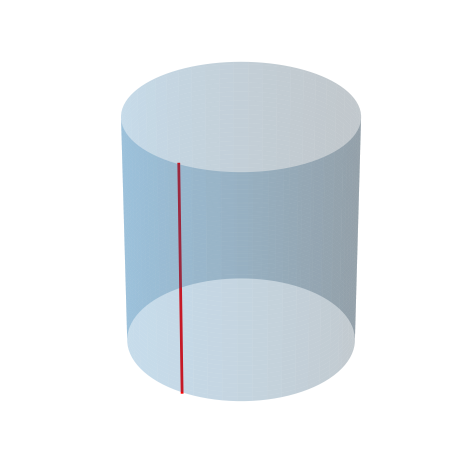
\includegraphics[width=0.9\textwidth]{images/cylinder_line.png}
 	  \caption{Vertical Line: case $b=0$}
	  \label{subfig:vertical}
	\end{subfigure}
	\hfill
	%------------------------------
	% Subfigure 2: Helix on the Cylinder
	\begin{subfigure}[b]{0.3\linewidth}
	  \centering
	  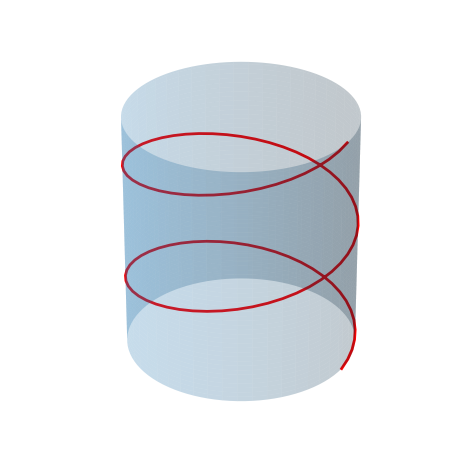
\includegraphics[width=0.9\textwidth]{images/cylinder_helix.png}
	  \caption{Helix: case $b\neq 0$}
	  \label{subfig:helix}
	\end{subfigure}
	\hfill
	%------------------------------
	% Subfigure 3: Horizontal Circle on the Cylinder
	\begin{subfigure}[b]{0.3\linewidth}
	  \centering
	  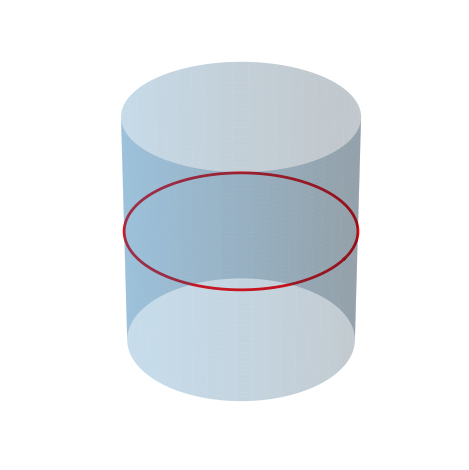
\includegraphics[width=0.9\textwidth]{images/cylinder_circle.png}
	  \caption{Circle: case $c=0$}
	  \label{subfig:circle}
	\end{subfigure}
	%------------------------------
	\caption{Geodesics on a Cylinder}
	\label{fig:geodesics-on-cylinder}
\end{figure}
  
\subsubsection{The Sphere}

We now consider the case of a sphere, which is a special case of a surface of revolution.
The sphere is a surface of revolution obtained by rotating a circle about an axis.
The parametric representation of the sphere is given by
\[
    \mathbf{r}(u, v) = \begin{bmatrix} R \cos (u) \cos (v) \\ R \cos (u) \sin (v) \\ R \sin (u) \end{bmatrix},
\]
where \(R\) is the radius of the sphere, \(u = \theta\) is the angle of rotation about the \(z\)-axis, and \(v = \phi\) is the angle of rotation about the \(x\)-axis.
The tangent vectors are given by
\[
    \mathbf{r}_u = \begin{bmatrix} -R \sin (u) \cos (v) \\ -R \sin (u) \sin (v) \\ R \cos (u) \end{bmatrix}, \quad \mathbf{r}_v = \begin{bmatrix} -R \cos (u) \sin (v) \\ R \cos (u) \cos (v) \\ 0 \end{bmatrix}.
\]
The metric for the sphere is given by
\[
    ds^2 = R^2 du^2 + R^2 \sin^2 (u) dv^2,
\]
Where the components of the metric tensor are given by \(E = R^2 \), \(F = 0\), and \(G = R^2 \sin^2 (u)\).
Thus the geodesic equations for the sphere are given by
\begin{align*}
    \ddot{u} + \sin(v) \cos(v) \dot{v}^2 &= 0 \\
    \ddot{v} + 2\tan(v) \dot{u} \dot{v} &= 0 
\end{align*}
The resulting system is a highly complex set of nonlinear differential equations, and in practice, geodesic equations are seldom solved directly.

This is where Clairaut's relation comes in handy.
We can use Clairaut's relation to simplify the geodesic equations.
We see that taking the derivatives of the metric tensor components with respect to \(v\) we have $E_v = 0$ and $G_v = 0$ which means that the sphere is a $u$-Clairaut parametrization.
Using Eq \eqref{eq:v_Clairaut_integral}, we get the following integral:
\[
    v = \pm \int \frac{c}{\sin(u)\sqrt{R^2\sin^{2}(u) - c^{2}}} \dd{u}
\]
We wont show the steps to solve this integral, as it is a bit tedious and not needed to understand the geodesic equations.
They can be found in full in \cite{oprea2007differential}, (Note: \cite{oprea2007differential} uses $v$-Clairaut parametrization, so the integration steps will slightly differ).
The solution to this integral is given by 
\[
\sin(v - d) = \lambda \cot(u)
\]
where \(d\) is a constant of integration and \(\lambda = \frac{c}{\sqrt{R^2 - c^2}}\).

Using the trigonometric identity \(\sin(v - d) = \sin(v)\cos(d) - \cos(v)\sin(d)\),  and find a common denominator $\sin(u)$ to get
\[
    \frac{\sin(v)\sin(u)}{\sin(u)}\cos(d) - \frac{\cos(v)\sin(u)}{\sin(u)}\sin(d) - \lambda \frac{\cos(u)}{\sin(u)} = 0
\]
If we substitute \(x = \cos(v)\sin(u), \quad y = \sin(v)\sin(u), \quad z = \cos(u)\), we can rewrite the equation as
\[
    y\cos(d) - x\sin(d) - \lambda z = 0
\]
Hence, the geodesic equations imply that the geodesics on the sphere lie on a plane \( ax + by + cz = d \) that passes through the origin.
So the geodesics on the sphere are great circles. Figure (\ref{fig:geodesics-on-sphere}) shows the geodesics on a sphere.

\begin{figure}[ht]
	\centering
	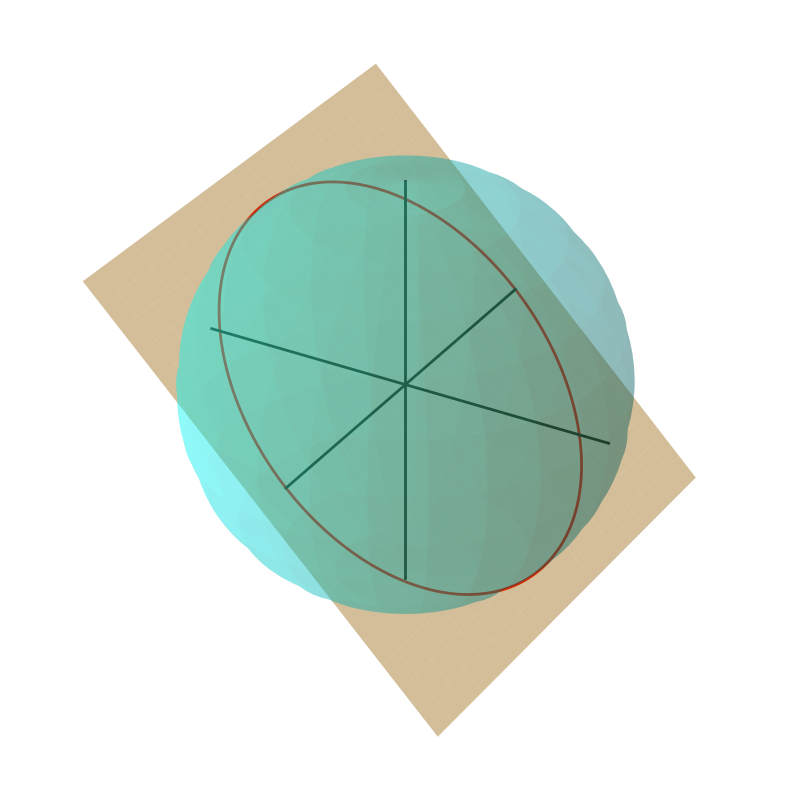
\includegraphics[width=0.4\textwidth]{images/sphere_circle_plane.png}
	\caption{Geodesics on a Sphere}
	\label{fig:geodesics-on-sphere}
\end{figure}

\subsubsection{The Hyperboloid}

Now we consider the case of a hyperboloid, which is a bit more complex to study than the sphere.
The hyperboloid is a surface of revolution obtained by rotating a hyperbola about an axis.
The parametric representation of the hyperboloid (also called a ”Hyperboloid of one sheet”) is given by
\[
    \mathbf{r}(u, v) = \begin{bmatrix} a \cosh (u) \cos (v) \\ a \cosh (u) \sin (v) \\ b \sinh (u) \end{bmatrix},
\]
where \(a\) and \(b\) are the semi-major and semi-minor axes of the hyperbola, respectively.

The tangent vectors are given by
\[
    \mathbf{r}_u = \begin{bmatrix} a \sinh (u) \cos (v) \\ a \sinh (u) \sin (v) \\ b \cosh (u) \end{bmatrix}, \quad \mathbf{r}_v = \begin{bmatrix} -a \cosh (u) \sin (v) \\ a \cosh (u) \cos (v) \\ 0 \end{bmatrix}.
\]
The metric for the hyperboloid is given by
\[
    ds^2 = ((a^2 + b^2)\sinh^{2}(u) + b^2) du^2 + a^2 \cosh^{2}(u) dv^2
\]
where \(E = (a^2 + b^2)\sinh^{2}(u) + b^2\), \(F = 0\), and \(G = a^2 \cosh^{2}(u)\).
Taking the derivatives of the components of the metric tensor, we find
\[
    E_u = 2(a^2 + b^2)\sinh(u)\cosh(u), \quad E_v = 0, \quad G_u = 2a^2 \sinh(u) \cosh(u), \quad G_v = 0.
\]
Thus, the hyperboloid is a $u$-Clairaut parametrization.
So the geodesic equations for the hyperboloid are given by
\begin{align*}
    \ddot{u} + \frac{(a^2 + b^2)\sinh(u)\cosh(u)}{(a^2 + b^2)\sinh^{2}(u) + b^2}\,\dot{u}^2 - \frac{a^2 \sinh(u) \cosh(u)}{(a^2 + b^2)\sinh^{2}(u) + b^2}\,\dot{v}^{2} &= 0 \\
    \ddot{v} + \tanh(u) \dot{u} \dot{v} &= 0
\end{align*}
Using Clairaut's relation, we can simplify the geodesic equations.
Since $E_v = 0$ and $G_v = 0$, we have a $u$-Clairaut parametrization for the hyperboloid.
Using Eq \eqref{eq:v_Clairaut_integral}, we get
\[
    v = \pm \int \frac{c\sqrt{(a^2 + b^2)\sinh^2(u) + b^2}}{a\cosh(u)\sqrt{a^2\cosh^2(u) - c^2}}\,\dd{u}
\]
Obviously, this integral is not trivial to solve, but we can use Clairaut's relation to analyze the geodesics on the hyperboloid.
We have that Clairaut's relation for the hyperboloid is given by
\[
    a \cosh(u) \sin(\phi) = C  
\]
As shown in \cite{khuangsatung2012geodesics}, by assuming that $u$ is very small number, we can consider the following cases:
\begin{itemize}
    \item If $C = 0$, then $\phi = 0$ and the geodesic corresponds to a meridian on the hyperboloid.
    \item If $C = a$ at $u = u_0 = 0$, then $\phi = \frac{\pi}{2}$ and the geodesic a parallel on the hyperboloid.
    \item If $\abs{C} < \abs{a}$, then $\phi$ is a constant angle and the geodesic is a helix on the hyperboloid.
\end{itemize}


\subsubsection{The Torus}

The torus is a surface of revolution obtained by rotating a circle about an axis that is not in the plane of the circle.
The parametric representation of the torus is given by
\[
    \mathbf{r}(u, v) = \begin{bmatrix} (R + r \cos (u)) \cos (v) \\ (R + r \cos (u)) \sin (v) \\ r \sin (u) \end{bmatrix},
\]
where \(R\) is the distance from the center of the torus to the center of the tube, and \(r\) is the radius of the tube.
The tangent vectors are given by
\[
    \mathbf{r}_u = \begin{bmatrix} -r \sin (u) \cos (v) \\ -r \sin (u) \sin (v) \\ r \cos (u) \end{bmatrix}, \quad \mathbf{r}_v = \begin{bmatrix} -(R + r \cos (u)) \sin (v) \\ (R + r \cos (u)) \cos (v) \\ 0 \end{bmatrix}.
\]
The metric for the torus is given by
\[
    ds^2 = r^2 du^2 + (R + r \cos (u))^2 dv^2,
\]
where \(E = r^2\), \(F = 0\), and \(G = (R + r \cos (u))^2\).
Taking the derivatives of the components of the metric tensor, we find
\[
    E_u = 0, \quad E_v = 0, \quad G_u = -2(R + r \cos (u))r \sin (u), \quad G_v = 0.
\]

Thus, the torus is a $u$-Clairaut parametrization.
So the geodesic equations for the torus are given by
\begin{align*}
    \ddot{u} + \frac{(R + r \cos (u))r \sin (u)}{r^2}\,\dot{u}^2 - \frac{(R + r \cos (u))^2}{r^2}\,\dot{v}^{2} &= 0 \\
    \ddot{v} + \frac{r \sin (u)}{R + r \cos (u)}\,\dot{u}\dot{v} &= 0
\end{align*}

Using Clairaut's relation, we can simplify the geodesic equations.
Using Eq \eqref{eq:v_Clairaut_integral}, we get
\[
    v = \pm \int \frac{cr}{(R + r \cos (u))\sqrt{(R + r \cos (u))^2 - c^2}}\,\dd{u}
\]
We can use Clairaut's relation to analyze the geodesics on the torus.
\[
    (R + r \cos (u)) \sin(\phi) = C
\]
By assuming that $u$ is very small number, therefore we will consider into 3 cases:

\begin{itemize}
    \item If $C = 0$, then $\phi = 0$ and the geodesic corresponds to a meridian on the torus.
    \item If $C = R + r$ at $u = u_0 = 0$, then $\phi = \frac{\pi}{2}$ and the geodesic a parallel on the torus.
    \item If $\abs{C} < \abs{R + r}$, then $\phi$ is a constant angle and the geodesic is a helix on the torus.
    % \item If $\abs{C} > \abs{R + r}$, then the geodesic is a closed curve on the torus.
\end{itemize}

\section{Symmetries, Isometries, and Killing Vector Fields}

Understanding the symmetries of a surface not only deepens our insight into its intrinsic geometry but also plays a crucial role in simplifying the computation of geodesics. 
In this section, we review the algebraic framework of continuous symmetries—embodied in the notion of a group—and then explain how these symmetries manifest as isometries on a surface. 
% Finally, we introduce Killing vector fields as the infinitesimal generators of continuous isometries, and we discuss how they lead to conserved quantities along geodesics.

\subsection{Groups and Continuous Symmetries}
Symmetries of a geometric object naturally form a mathematical structure called a \emph{group}. 
Informally, a group is a collection of operations (such as rotations, translations, or reflections) that can be combined (via composition) while preserving the object’s essential properties. 
More formally, we recall the following definition.

\begin{definition}[Group]
	A set $G$ equipped with a binary operation $\circ: G \times G \to G$ is called a \emph{group} if the following properties hold:
	\begin{enumerate}
	    \item (\textbf{Closure}) For all $a,b \in G$, the product $a \circ b$ is also in $G$.
	    \item (\textbf{Associativity}) For all $a,b,c \in G$, $(a \circ b) \circ c = a \circ (b \circ c)$.
	    \item (\textbf{Identity}) There exists an element $e \in G$ such that $e \circ a = a \circ e = a$ for every $a \in G$.
	    \item (\textbf{Inverses}) For every $a \in G$, there exists an element $a^{-1} \in G$ satisfying $a \circ a^{-1} = a^{-1} \circ a = e$.
	\end{enumerate}
\end{definition}

Examples of groups include the set of integers under addition, the set of non-zero real numbers under multiplication, and the set of rotations in three-dimensional space.


A manifold, such as a surface $\mathcal{S}$, possesses a symmetry if there exists a diffeomorphism (a smooth, invertible map) $\phi: \mathcal{S} \to \mathcal{S}$ from the manifold to itself that preserves the geometric structure.
This means that the metric tensor $g$ remains invariant under the transformation:
\[
	\phi \circ g = g,
\]
The set of all such diffeomorphisms forms a group, called the \emph{symmetry group} of the manifold.

% \subsubsection{Lie Groups}
% A Lie group is a group that is also a smooth manifold, so its operations are smooth. For example, 
% the rotation group $SO(3)$, $SL(2,\mathbb{R})$, and the Poincaré group are Lie groups. 
% Their associated Lie algebras—tangent spaces at the identity—capture the infinitesimal generators of the group.

\subsubsection{Generators of a Group}
Another important concept is the idea of generators of a group.
A generator of a group is an element that can be used to produce all other elements of the group through repeated application of the group operation.

\begin{definition}[Generator]
	Let $G$ be a group. An element $g \in G$ is called a \emph{generator} of the group if every element of $G$ can be expressed as a power of $g$, i.e., for every $h \in G$, there exists an integer $n$ such that $h = g^n$.
	\[
		G = \langle g \rangle = \{ g^n \mid n \in \R \}
	\]
\end{definition}


In the context of continuous symmetries, we can think of a generator as an infinitesimal transformation that generates a one-parameter group of transformations.
For example, the rotation group in three-dimensional space can be generated by a single rotation about a fixed axis.
The generators of a group can be thought of as the "building blocks" of the group, and they play a crucial role in understanding the structure and properties of the group.


\subsection{Isometries on Surfaces}
Given a surface $\mathcal{S}$ with a metric $g$, an \emph{isometry} is a transformation that preserves distances. More precisely, a bijective map
\[
f: S \to S
\]
is an \emph{isometry} if, for all points $p,q\in S$, the distance between $p$ and $q$ equals the distance between their images:
\[
d\big(f(p),f(q)\big)=d(p,q).
\]
This invariance implies that the local expressions for the metric coefficients remain unchanged under the transformation. 
For example, on a round sphere the full isometry group is the orthogonal group $O(3)$, while for the Euclidean plane both rotations and translations are isometries.

It is important to note that isometries preserve geodesics; if $\gamma$ is a geodesic on $S$, then so is $f\circ\gamma$. 
This property will be key when we introduce the infinitesimal generators of continuous isometries.


\subsection{Killing Vector Fields}
A Killing vector field is a vector field on a manifold that generates an isometry of the metric.

\begin{definition}[Killing Vector Field]
	Let \(M\) be a manifold with metric \(g\). A vector field \(K\) on \(M\) is called a \emph{Killing vector field} if the Lie derivative of the metric with respect to \(K\) vanishes:
	\[
		\mathcal{L}_{K} (g) = 0.
	\]
	This means that the flow generated by \(K\) preserves the metric, and hence the distances and angles on the manifold.
\end{definition}
The Lie derivative of the metric with respect to a vector field \(K\) is given by
\[
	\mathcal{L}_{K} (g_{\mu\nu}) = \nabla_{\mu} K^{\mu} + \nabla_{\nu} K^{\nu},
\]
Where \(\nabla\) is the covariant derivative associated with the metric \(g\).
We wont go into details of what the Lie derivative is, but it is a way to measure how a tensor field changes along the flow of a vector field.
For more details, see \cite{oprea2007differential},\cite{note32020covariant},\cite{atkins2018solving},\cite{carrol2019spacetime}.


Easiest way to find a Killing vector field is to look for symmetries of the metric.
That is, we want to find the coordinates of which the metric is independent off and thus the metric is invariant under the transformation of such coordinates.

For example, let us consider the following metric:
\[
	ds^{2} = dr^{2} + r^{2}d\theta^{2} 
\]
This metric is independent of the coordinate \(\theta\), so we can find a Killing vector corresponding to the isometry generated by rotations about the axis of revolution.
The Killing vector field is given by
\[
	\xi^{1} = \frac{\partial}{\partial \theta} = \begin{bmatrix} 0 \\ 1 \end{bmatrix}
\]
This vector field generates a rotation about the axis of revolution, and it is a Killing vector field because it preserves the metric.
In general, a Killing vector field is a vector field that generates an isometry of the metric.


As shown in \cite{carrol2019spacetime} and \cite{atkins2018solving}, if $K^{\mu}$ is a Killing vector field, then we have the following to holds
\begin{equation}\label{eq:Killing_vector}
	\text{const} = g_{\mu\nu}K^{\mu}\dv{x^{\nu}}{t} 
\end{equation}
Additionally, we have another constant for the motion along the geodesic, which is given by
\begin{equation}\label{eq:epsilon_equation}
	\epsilon = - \sum_{\mu,\nu} g_{\mu\nu}\dv{x^{\mu}}{t}\dv{x^{\nu}}{t}
\end{equation}
In the context of general relativity, this equation describes the motion of a test particle in a gravitational field where \(\epsilon = 0\) for null geodesics, \(\epsilon = 1\) for time-like geodesics, and \(\epsilon = -1\) for space-like geodesics.

\subsection{Clairaut's Relation from Killing Vector Fields}

Consider a surface of revolution obtained by rotating a profile curve around an axis, with local coordinates $(u,v)$ so that the induced metric reads
$$
ds^2 \;=\; du^2 \;+\; f(u)^2\,dv^2\,,
$$
where $f(u)$ is the distance from the axis.

Because the metric coefficients do not depend on $v$, the vector field

$$
K = \frac{\partial}{\partial v}
$$

is Killing (it generates rotations about the axis).

Applying the general conservation law $g(K,\dot x)=\text{const}$ gives

$$
g\bigl(\dot x,\partial_v\bigr)
= f(u)^2\,\frac{dv}{d\lambda}
= L,
$$
where $L$ is the conserved “angular momentum.”

For a unit-speed geodesic one has

$$
\underbrace{\Bigl(\frac{du}{d\lambda}\Bigr)^2}_{=\,(\cos\psi)^2}
\;+\;
\underbrace{f(u)^2\Bigl(\frac{dv}{d\lambda}\Bigr)^2}_{=\,(\sin\psi)^2}
=1,
$$

so we define the angle $\psi$ between the geodesic and a meridian by

$$
\cos\psi = \frac{du}{d\lambda},
\qquad
\sin\psi = f(u)\,\frac{dv}{d\lambda}.
$$

Hence
$$
f(u)\,\sin\psi
= f(u)\;f(u)\,\frac{dv}{d\lambda}
= L,
$$

\subsection{Noether's Theorem}
Noether's theorem reveals that every continuous symmetry of the action leads to a conserved quantity. 
In a system described by a Lagrangian \( \mathcal{L} \), if the action is invariant under a continuous transformation, then there exists a corresponding conserved current.

For instance, consider the following standard symmetries:
\begin{itemize}
    \item Invariance under time translations implies conservation of energy.
    \item Invariance under spatial translations implies conservation of linear momentum.
    \item Invariance under rotations implies conservation of angular momentum.
\end{itemize}

In the study of geodesics, if the metric (or Lagrangian) remains invariant under a continuous transformation generated by a Killing vector field \( K \), then the quantity
\[
    g_{\mu\nu}K^{\mu}\frac{dx^{\nu}}{d\lambda}
\]
remains constant along the geodesic (with \( \lambda \) as an affine parameter). 
This conserved quantity is fundamental in reducing and solving the geodesic equations, as seen in Clairaut's relation for surfaces of revolution, where the projection of the tangent vector onto the symmetry direction is preserved.

\section{A look to Black Holes Geodesics}

In this section, we will look at the geodesics of a black hole.
We will use the Schwarzschild metric, which describes the spacetime geometry outside a spherically symmetric, non-rotating mass. The Schwarzschild metric is given by
\begin{equation}\label{eq:schwarzschild_metric}
	ds^2 = -\left(1 - \frac{2GM}{r}\right) dt^2 + \left(1 - \frac{2GM}{r}\right)^{-1} dr^2 + r^2 d\Omega^2
\end{equation}
where 
\[
d\Omega^2 = d\theta^2 + \sin^2(\theta) d\phi^2
\] 
is the metric on the unit sphere, \(G\) is the gravitational constant, \(M\) is the mass of the black hole, and \(c = 1\) is the speed of light under natural units.
The Schwarzschild metric is a solution to the Einstein field equations in general relativity and describes the spacetime geometry around a non-rotating, spherically symmetric black hole.

Because the Schwarzschild metric is a spherically symmetric solution, we can choose to study the geodesics in the equatorial plane, where \(\theta = \frac{\pi}{2}\).
This simplifies the metric to
\begin{equation}\label{eq:schwarzschild_metric_equatorial}
	ds^2 = -\left(1 - \frac{2GM}{r}\right) dt^2 + \left(1 - \frac{2GM}{r}\right)^{-1} dr^2 + r^2 d\phi^2
\end{equation}
This in turn converts our metric from a 4D metric to a 3D metric, for which we can use to visualize the geodesics in 2D.
The metric tensor is given by
\[
	g_{\mu\nu} = \begin{bmatrix}
	-\left(1 - \frac{2GM}{r}\right) & 0 & 0 \\
	0 & \left(1 - \frac{2GM}{r}\right)^{-1} & 0 \\
	0 & 0 & r^2
	\end{bmatrix}
\]
Because the metric is independent of the coordinates \(t\) and \(\phi\), we can use the Killing vector fields associated with these symmetries to find conserved quantities along the geodesics.
The Killing vector fields associated with the Schwarzschild metric are given by
\begin{align*}
	\xi^{1} &= \frac{\partial}{\partial t} = \begin{bmatrix} 1 \\ 0 \\ 0 \end{bmatrix} \\
	\xi^{3} &= \frac{\partial}{\partial \phi} = \begin{bmatrix} 0 \\ 0 \\ 1 \end{bmatrix}
\end{align*}
The conserved quantities associated with these Killing vector fields are given by
\begin{align}
	E &= -g_{11} \, \xi^{1} \, \dv{x^{1}}{\lambda} = \left(1 - \frac{2GM}{r}\right) \dv{t}{\lambda} \label{eq:energy} \\
	L &= g_{33} \, \xi^{3} \, \dv{x^{3}}{\lambda} = r^2 \dv{\phi}{\lambda} \label{eq:angular_momentum}
\end{align}
where \(E\) is the energy of the particle and \(L\) is the angular momentum of the particle.

Pluggin this into Eq.(\ref{eq:epsilon_equation}), we get
\begin{align*}
	\epsilon &= -g_{\mu\nu}\dv{x^{\mu}}{t}\dv{x^{\nu}}{t} = -g_{tt} \left(\dv{t}{\lambda}\right)^2 - g_{rr} \left(\dv{r}{\lambda}\right)^2 - g_{\phi\phi} \left(\dv{\phi}{\lambda}\right)^2 \\
	&= -\left(1 - \frac{2GM}{r}\right) \left(\dv{t}{\lambda}\right)^2 - \left(1 - \frac{2GM}{r}\right)^{-1} \left(\dv{r}{\lambda}\right)^2 - r^2 \left(\dv{\phi}{\lambda}\right)^2
\end{align*}

Moving $\epsilon$ to the other side, and multiplying by $g_{tt}$, we get
\[
	0 = \left(1 - \frac{2GM}{r}\right)^{2} \left(\dv{t}{\lambda}\right)^2 + \left(\dv{r}{\lambda}\right)^2 + \left(1 - \frac{2GM}{r}\right) \left(r^2 \left(\dv{\phi}{\lambda}\right)^2 + \epsilon \right)
\]
Substituting the expressions for \(E\) and \(L\) from Eq.(\ref{eq:energy}) and Eq.(\ref{eq:angular_momentum}), we get
\begin{equation}
	0 = -E^{2} + \left(\dv{r}{\lambda}\right)^2 + \left(1 - \frac{2GM}{r}\right) \left(\frac{L^{2}}{r^{2}} + \epsilon \right)
\end{equation}

Expanding the last term and dividing by $2$, we get
\[
	\frac{1}{2} \left(\dv{r}{\lambda}\right)^2 + \frac{1}{2} \left(1 - \frac{2GM}{r}\right) \left(\frac{L^{2}}{r^{2}} + \epsilon \right) = \frac{E^{2}}{2}
\]
This is the effective potential for the Schwarzschild metric, and it describes the motion of a particle in the gravitational field of a black hole.
The effective potential is given by
\begin{equation}
	V_{\text{eff}}(r) = \left(1 - \frac{2GM}{r}\right) \left(\frac{L^{2}}{r^{2}} + \epsilon \right) = \epsilon - \epsilon\frac{2GM}{r} + \frac{L^{2}}{r^{2}} - \frac{2GM L^{2}}{r^{3}}
\end{equation}
The effective potential describes the motion of a particle in the gravitational field of a black hole, and it can be used to analyze the stability of orbits around the black hole.

\subsection{Schwarzschild Radius}
For a black hole, with some mass \(M\), its event horizon (i.e. the surface beyond which nothing can escape) is located at the Schwarzschild radius, which is given by
\[
	r_{s} = \frac{2GM}{c^{2}} = 2GM
\]
with \(c = 1\) in natural units.
The Schwarzschild radius is the radius of the event horizon of a black hole, and it is the point at which the gravitational pull of the black hole becomes so strong that nothing, not even light, can escape from it.
\subsection{Circular Orbits}
Circular orbits are a special case of geodesics in the Schwarzschild metric, where the radial coordinate \(r\) is constant.
We find a circular orbit at $r = r_{c}$ that satisfies the following:
\[
	\dv{V_{\text{eff}}}{r}\Bigg|_{r_{c}} = 0
\]
Taking the derivative of the effective potential, we get
\begin{equation}\label{eq:dV_eff}
	\dv{V_{\text{eff}}}{r}\Bigg|_{r_{c}} = \frac{2GM\epsilon}{r_{c}^{2}} - \frac{2L^{2}}{r_{c}^{3}} + \frac{6GM L^{2}}{r_{c}^{4}}
\end{equation}
Multiplying by $r_{c}^{4}/2$, we get
\[
	0 = GM\epsilon r_{c}^{2} - L^{2} r_{c} + 3GM L^{2}
\]

\subsection{Null Geodesics}

In Newtonian gravity, only massive objects feel the gravitational attraction of other masses, so massless particles like photons travel along straight lines in a flat spacetime described by the Minkowski metric \cite{carrol2019spacetime}.  
By contrast, in general relativity gravity is encoded as curvature of spacetime around a mass, and light rays follow this curvature.  
Because photons trajectories are not affected by the mass of the object they are passing by, and thus must follow straight lines in the curved spacetime, we can use the geodesic equations to describe their motion.
These light‐ray trajectories are called \emph{null geodesics}, characterized by \ref{eq:epsilon_equation} with \(\epsilon = 0\).

For circular null orbits in the Schwarzschild metric, we set \(\epsilon=0\) in equation \ref{eq:dV_eff} gives
\[
0 \;=\; -\,L^{2}\,r_{c} \;+\; 3\,G\,M\,L^{2},
\]
where \(L\) is the photon’s conserved angular momentum per unit energy.  
Solving for \(r_{c}\) yields
\[
r_{c} \;=\; 3\,G\,M.
\]
This special radius \(r_{c}\) defines the \emph{photon sphere}—the locus where light can orbit the black hole in an unstable circular path. 
Any small radial perturbation will cause the photon to either spiral inward into the black hole or escape back to infinity.

We see that the photon sphere is located relatively close to the event horizon of the black hole, seperated by a factor of \(GM\).


\subsection{Time-like Geodesics}
For time-like geodesics, we have \(\epsilon = 1\), so we can rewrite the equation as
\[
	0 = GM r_{c}^{2} - L^{2} r_{c} + 3GM L^{2}
\]
This is a quadratic equation in \(r_{c}\), and we can use the quadratic formula to find the radius of the circular orbit:
\[
	r_{c} = \frac{L^{2} \pm \sqrt{L^{4} - 12GM L^{2}}}{2GM}
\]
This gives us two solutions for the radius of the circular orbit, one of which is stable and the other is unstable.
The stable solution is given by
\[
	r_{c} = \frac{L^{2} + \sqrt{L^{4} - 12GM L^{2}}}{2GM}
\]
The unstable solution is given by
\[
	r_{c} = \frac{L^{2} - \sqrt{L^{4} - 12GM L^{2}}}{2GM}
\]
The stable solution corresponds to a circular orbit that is stable under small perturbations, while the unstable solution corresponds to a circular orbit that is unstable under small perturbations.

% \color{black}
\section{Conclusion}

\section{References}

\nocite{*}
\bibliographystyle{unsrt}
\bibliography{references}


\end{document}